\documentclass{article}
\usepackage{graphicx}
\usepackage{float}
\usepackage{caption}
\usepackage{subcaption}
\usepackage{gensymb}
\usepackage[utf8]{inputenc}
\usepackage[a4paper, total={6in, 8in}]{geometry}

\renewcommand{\thesubsection}{\thesection.\alph{subsection}}

\begin{document}

\author{Antonella Dellanzo}
\title{Guía 2 - Introducción al procesamiento digital de imágenes}
\date{}
\maketitle

\section{RGB Y HSI}


\subsection{}
El archivo correspondiente a este inciso se llama \textbf{histogramasDeImagenRGB.m} y toma como parámetro de entrada una imagen que tenga tres canales (se realiza este chequeo) y genera tres figuras correspondientes a los histogramas a los canales R, G y B. Por ejemplo, al ejecutarlo con la imagen llamada \textit{1923xx.png}, se obtuvieron los siguientes resultados:

\begin{figure}[H]
	\begin{subfigure}{0.5\textwidth}
	\centering
        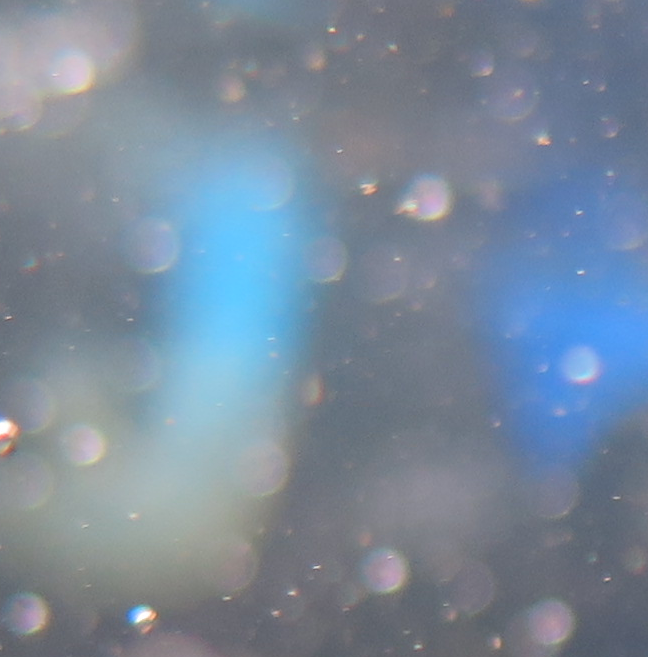
\includegraphics[scale=0.4]{1923xx.png}
    \subcaption{Imagen original}
    \end{subfigure}\hfill
    \begin{subfigure}{0.5\textwidth}
        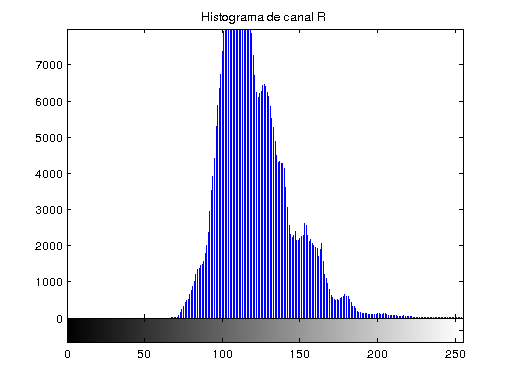
\includegraphics[width=0.9\textwidth]{histogramaR-1923.png}
    \subcaption{Histograma de canal R}
    \end{subfigure}\hfill
    \begin{subfigure}{0.5\textwidth}
        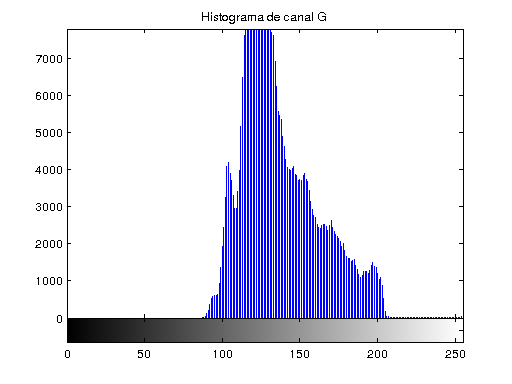
\includegraphics[width=0.9\textwidth]{histogramaG-1923.png}
    \subcaption{Histograma de canal G}
    \end{subfigure}\hfill
    \begin{subfigure}{0.5\textwidth}
        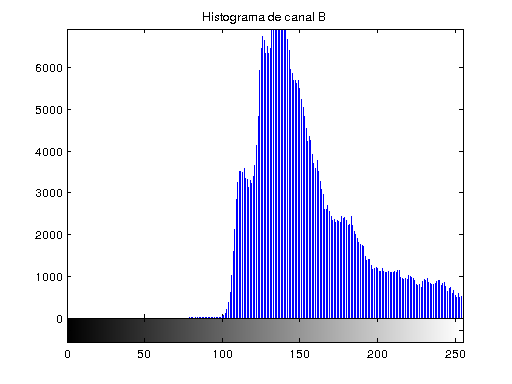
\includegraphics[width=0.9\textwidth]{histogramaB-1923.png}
    \subcaption{Histograma de canal B}
    \end{subfigure}
\end{figure}

\subsection{}

El archivo correspondiente a este inciso se llama \textbf{ecualizacionesDeRGB.m} y toma como parámetro de entrada una imagen que tenga tres canales y sean enteros de 8 bits (caso contrario lanza una excepción). Como resultado genera dos figuras: la primera con la imagen original y cada canal ecualizado por separado; y la segunda muestra una imagen nueva con estos tres nuevos canales ecualizados. 

Por ejemplo, al ejecutarlo con la imagen llamada \textit{1908xx.png}, se obtuvieron los siguientes resultados:

\begin{figure}[H]
	\begin{subfigure}{0.5\textwidth}
	\centering
        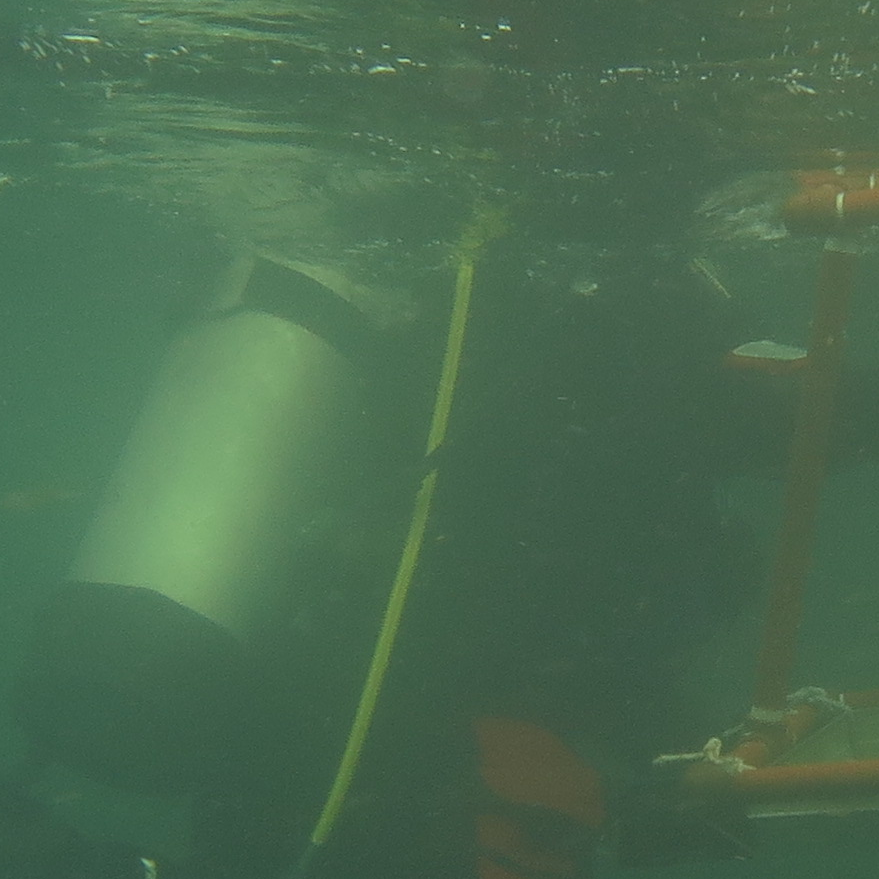
\includegraphics[scale=0.5]{1908xx.png}
    \subcaption{Imagen original}
    \end{subfigure}\hfill
	\begin{subfigure}{0.5\textwidth}
	\centering
        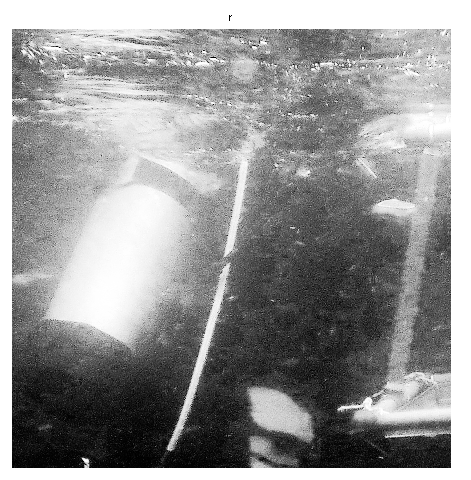
\includegraphics[width=0.9\textwidth]{1908xx-ecualizacion-r.png}
    \subcaption{Canal R ecualizado}
    \end{subfigure}\hfill
	\begin{subfigure}{0.5\textwidth}
	\centering
        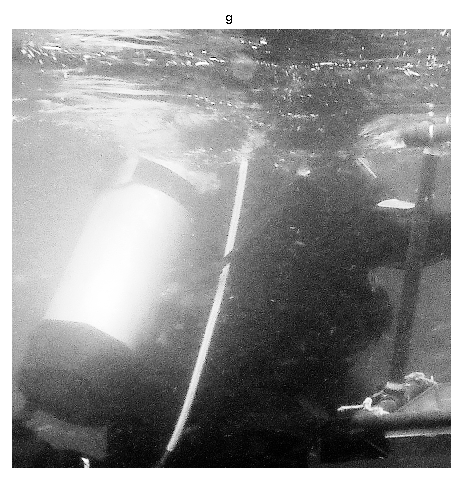
\includegraphics[width=0.9\textwidth]{1908xx-ecualizacion-g.png}
    \subcaption{Canal G ecualizado}
    \end{subfigure}\hfill
	\begin{subfigure}{0.5\textwidth}
	\centering
        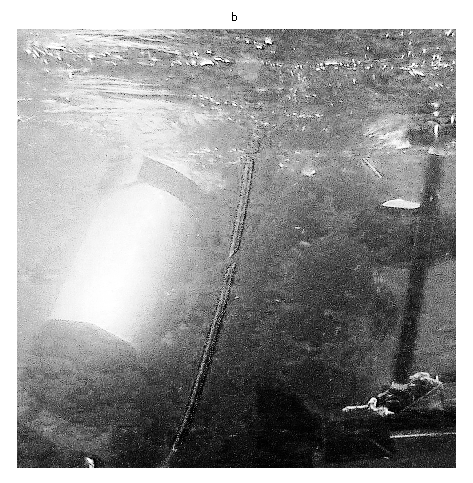
\includegraphics[width=0.9\textwidth]{1908xx-ecualizacion-b.png}
    \subcaption{Canal B ecualizado}
    \end{subfigure}\hfill
	\centering
	\begin{subfigure}{0.5\textwidth}
	\centering
        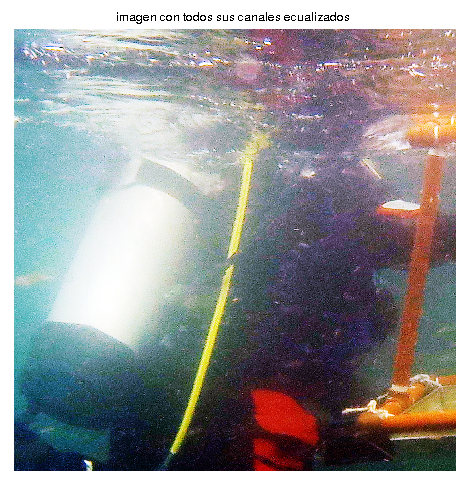
\includegraphics[width=0.9\textwidth]{1908xx-con-canales-ecualizados.png}
    \subcaption{Imagen final con todos sus canales ecualizados}
    \end{subfigure}\hfill
\end{figure}

\subsection{}

El archivo correspondiente a este inciso se llama \textbf{rgbToHsi.m} y toma dos parámetros de entrada: la imagen y un booleano que indica si se desea generar una figura que muestra la imagen final en formato HSI, el canal H, el canal S y el canal I. La función devuelve la nueva imagen en HSI.

El problema con el que me encontré en la resolución de este inciso fue que, al intentar obtener los canales Hue y Saturación, estaba realizando una división por cero y me quedaban valores no válidos en la matriz. Si bien en la imagen final en HSI esto no era notorio, al realizar luego la transformación de HSI a RGB perdía píxeles de la imagen, los cuales quedaban negros. Para solucionar esto, siempre que realizo una división, me aseguro de que haya un valor mayor a cero. Para esto, matlab cuenta con una función que devuelve el mínimo valor de double (\textit{realmin('double')}).

Por ejemplo, al ejecutarlo con la imagen llamada \textit{1901xx.png}, se obtuvieron los siguientes resultados:

\begin{figure}[H]
	\begin{subfigure}{0.5\textwidth}
	\centering
        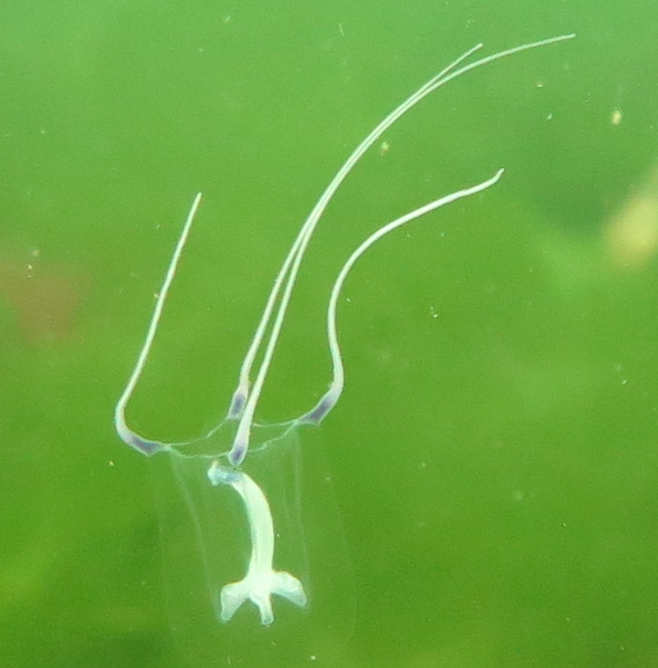
\includegraphics[width=0.7\textwidth]{1901xx.png}
    \subcaption{Imagen original}
    \end{subfigure}\hfill
	\begin{subfigure}{0.5\textwidth}
	\centering
        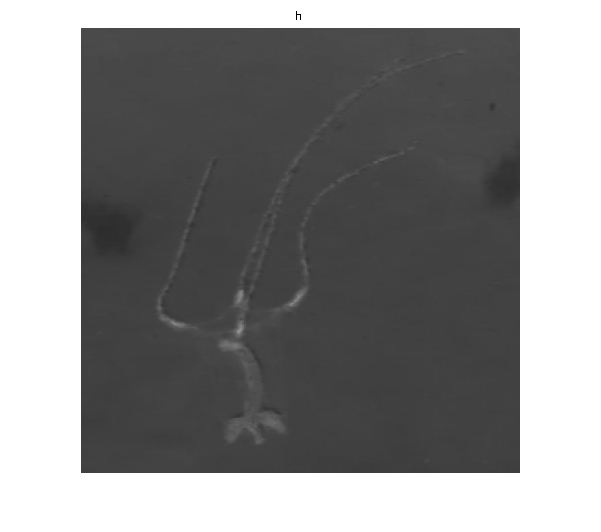
\includegraphics[width=0.9\textwidth]{1901-hsi-h.png}
    \subcaption{Canal H}
    \end{subfigure}\hfill
	\begin{subfigure}{0.5\textwidth}
	\centering
        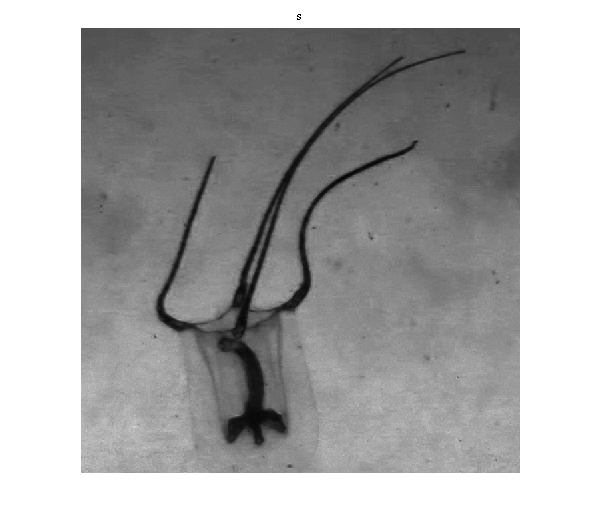
\includegraphics[width=0.9\textwidth]{1901-hsi-s.png}
    \subcaption{Canal S}
    \end{subfigure}\hfill
	\begin{subfigure}{0.5\textwidth}
	\centering
        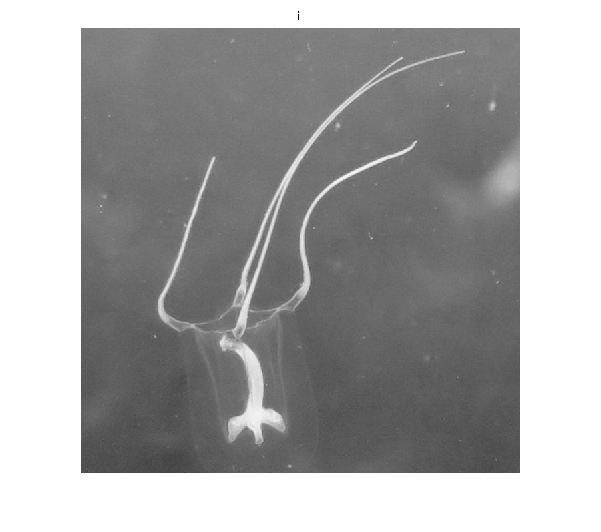
\includegraphics[width=0.9\textwidth]{1901-hsi-i.png}
    \subcaption{Canal I}
    \end{subfigure}\hfill
	\centering
	\begin{subfigure}{0.5\textwidth}
	\centering
        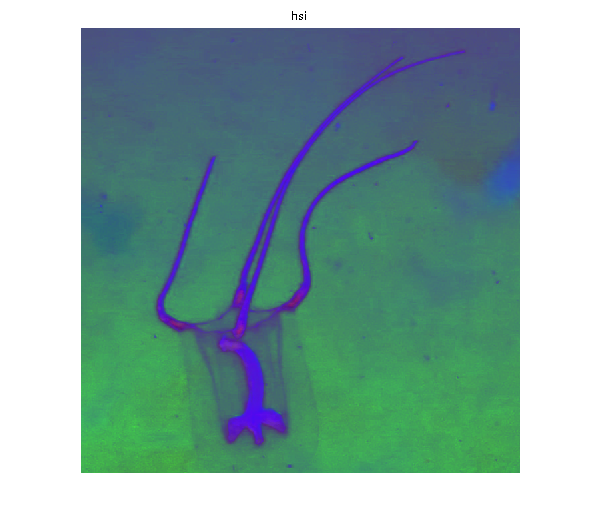
\includegraphics[width=0.9\textwidth]{1901-hsi.png}
    \subcaption{Imagen final en formato hsi}
    \end{subfigure}\hfill
\end{figure}

\subsection{}

Para este ejercicio se encuntran dos archivos:
\begin{itemize}
\item \textbf{ecualizarIDeHsiYTransformarEnRGB.m}: Toma como parámetro de entrada una imagen en RGB (se realizan los chequeos correspondientes de que tenga 3 canales y sea una matriz de enteros de 8 bits) y 
genera una figura en la que se muestra la imagen original, la imagen en hsi, la imagen en hsi con el canal I ecualizado y la imagen final (la cual se retorna en la función) en RGB que se generó luego de ecualizar el canal I.
\item \textbf{hsiToRgb.m}: Toma como parámetro de entrada una imagen en hsi que debe ser de 3 canales y de doubles, y un booleano que indica si se desea generar una figura que muestra la nueva imagen en RGB, junto con sus canales R, G y B.
\end{itemize}

Por ejemplo, al ejecutarlo con la imagen llamada \textit{1892xxx.png}, se obtuvieron los siguientes resultados:

\begin{figure}[H]
	\begin{subfigure}{0.5\textwidth}
	\centering
        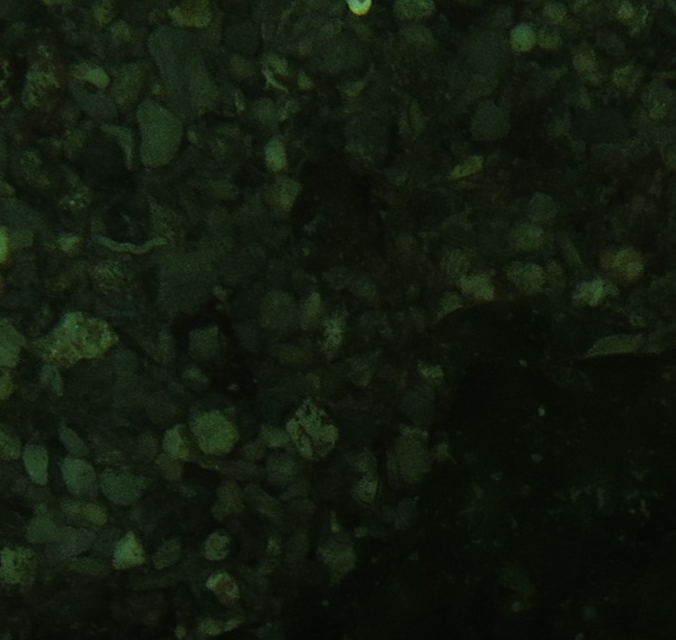
\includegraphics[scale=0.5]{1892xxx.png}
    \subcaption{Imagen original}
    \end{subfigure}\hfill
	\begin{subfigure}{0.5\textwidth}
	\centering
        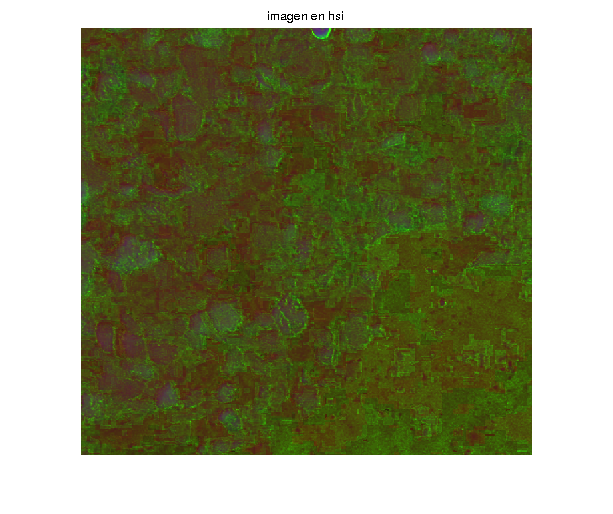
\includegraphics[width=0.9\textwidth]{1892xxx-hsi.png}
    \subcaption{Imagen en hsi}
    \end{subfigure}\hfill
	\begin{subfigure}{0.5\textwidth}
	\centering
        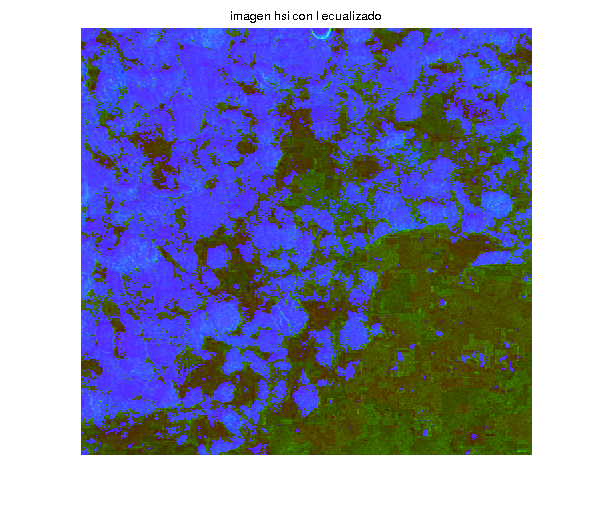
\includegraphics[width=0.9\textwidth]{1892xxx-hsi-i-ecualizado.png}
    \subcaption{Imagen en hsi con I ecualizado}
    \end{subfigure}\hfill
	\begin{subfigure}{0.5\textwidth}
	\centering
        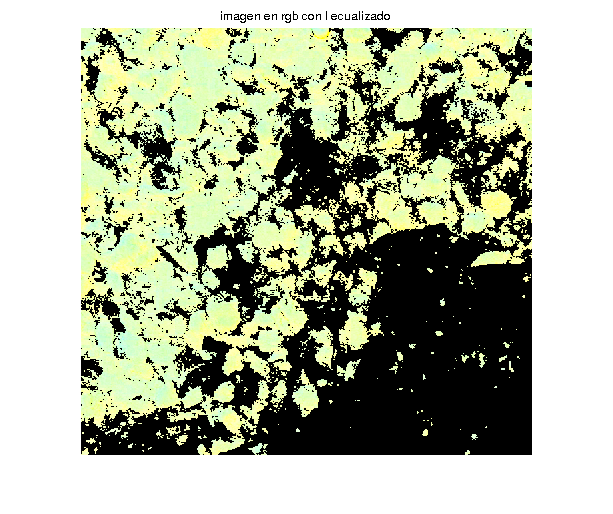
\includegraphics[width=0.9\textwidth]{1892xxx-rgb-i-ecualizado.png}
    \subcaption{Imagen en RGB con canal I ecualizado}
    \end{subfigure}\hfill
\end{figure}

\subsection{}

El archivo correspondiente a este inciso se llama \textbf{aplicarTransformacionesACadaCanal.m} y toma como parámetro de entrada una imagen en RGB y genera tres figuras:
\begin{itemize}
\item Muestra la imagen en HSI junto con cada uno de sus canales luego de las transformaciones
\item Muestra la imagen original en RGB y la nueva imagen en RGB luego de aplicadas las transformaciones correspondientes en los canales HSI
\item Muestra la imagen RGB final (la cual además se retorna de la función)
\end{itemize} 

El archivo final entregado genera solo una de las posibles transformaciones. 
A continuación presento ejemplos de imágenes finales en RGB con distintas transformaciones aplicadas a cada canal (en cada imagen aclaro las transformaciones aplicadas a cada canal):

\begin{figure}[H]
	\begin{subfigure}{0.5\textwidth}
	\centering
        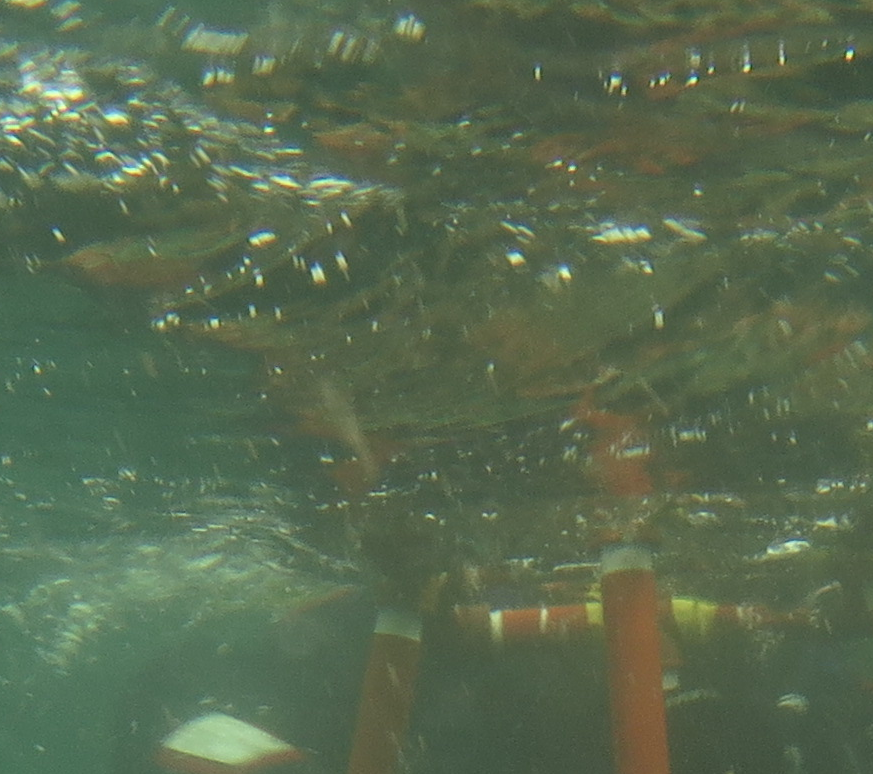
\includegraphics[scale=0.5]{1908iv.png}
    \subcaption{Imagen original}
    \end{subfigure}\hfill
	\begin{subfigure}{0.5\textwidth}
	\centering
        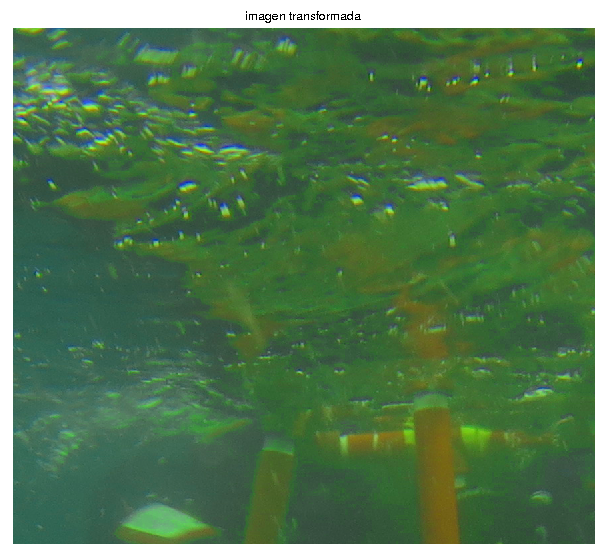
\includegraphics[width=0.9\textwidth]{1098iv-transformada-20-2x-log.png}
    \subcaption{Imagen transformada aumentando $20\degree$ H, multiplicado por 2 a S y aplicando log(1 + I) a I}
    \end{subfigure}\hfill
\end{figure}\hfill

\begin{figure}[H]
	\begin{subfigure}{0.5\textwidth}
	\centering
        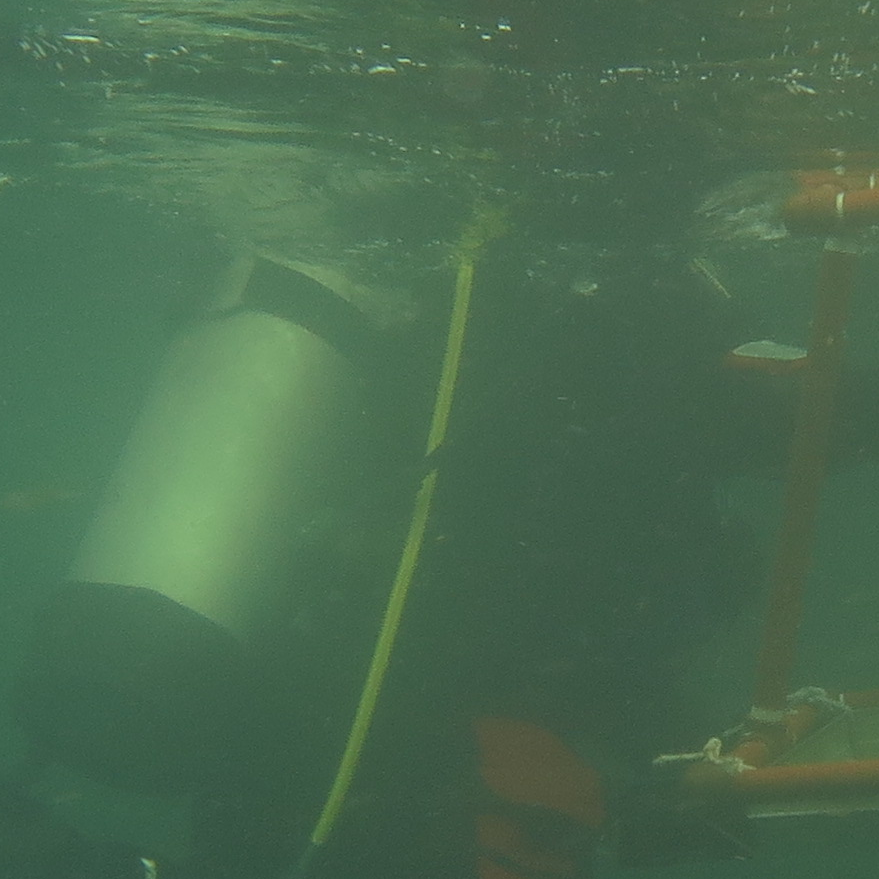
\includegraphics[scale=0.5]{1908xx.png}
    \subcaption{Imagen original}
    \end{subfigure}\hfill
	\begin{subfigure}{0.5\textwidth}
	\centering
        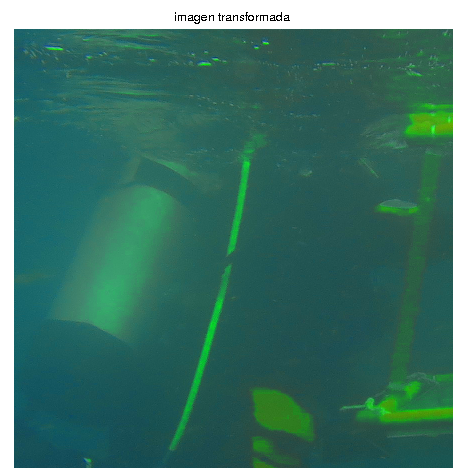
\includegraphics[width=0.9\textwidth]{1908xx-transformada-40-3x-log.png}
    \subcaption{Imagen transformada aumentando $40\degree$ H, multiplicado por 3 a S y aplicando log(1 + I) a I}
    \end{subfigure}\hfill
\end{figure}\hfill

\begin{figure}[H]
	\begin{subfigure}{0.5\textwidth}
	\centering
        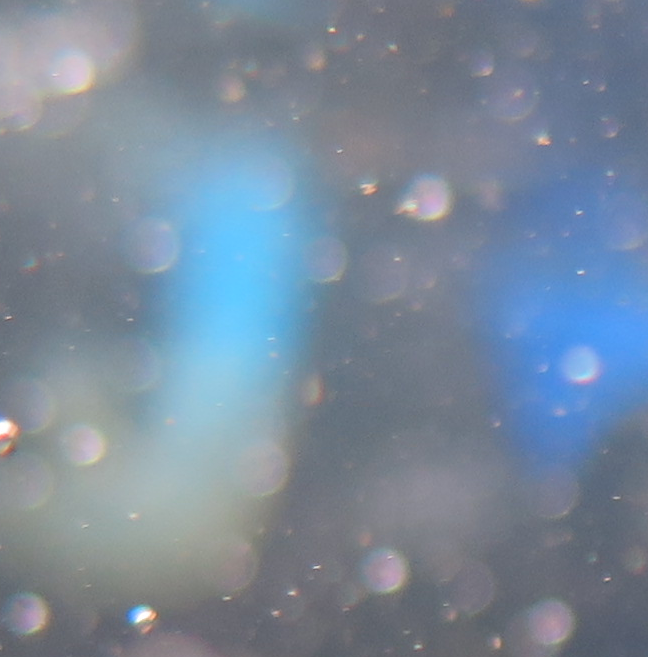
\includegraphics[scale=0.7]{1923xx.png}
    \subcaption{Imagen original}
    \end{subfigure}\hfill
	\begin{subfigure}{0.5\textwidth}
	\centering
        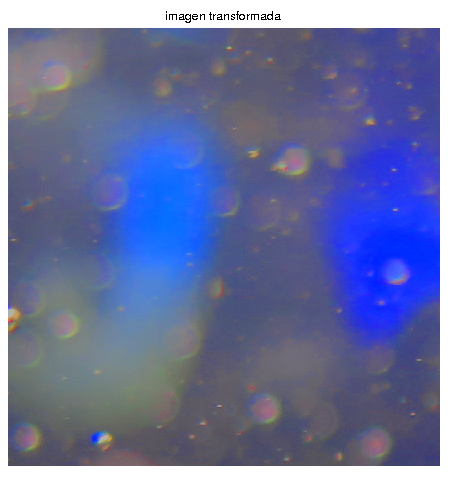
\includegraphics[width=0.9\textwidth]{1923-transformada-20-2x-log.png}
    \subcaption{Imagen transformada aumentando $20\degree$ H, multiplicado por 2 a S y aplicando log(1 + I) a I}
    \end{subfigure}\hfill
\end{figure}\hfill

\begin{figure}[H]
	\begin{subfigure}{0.5\textwidth}
	\centering
        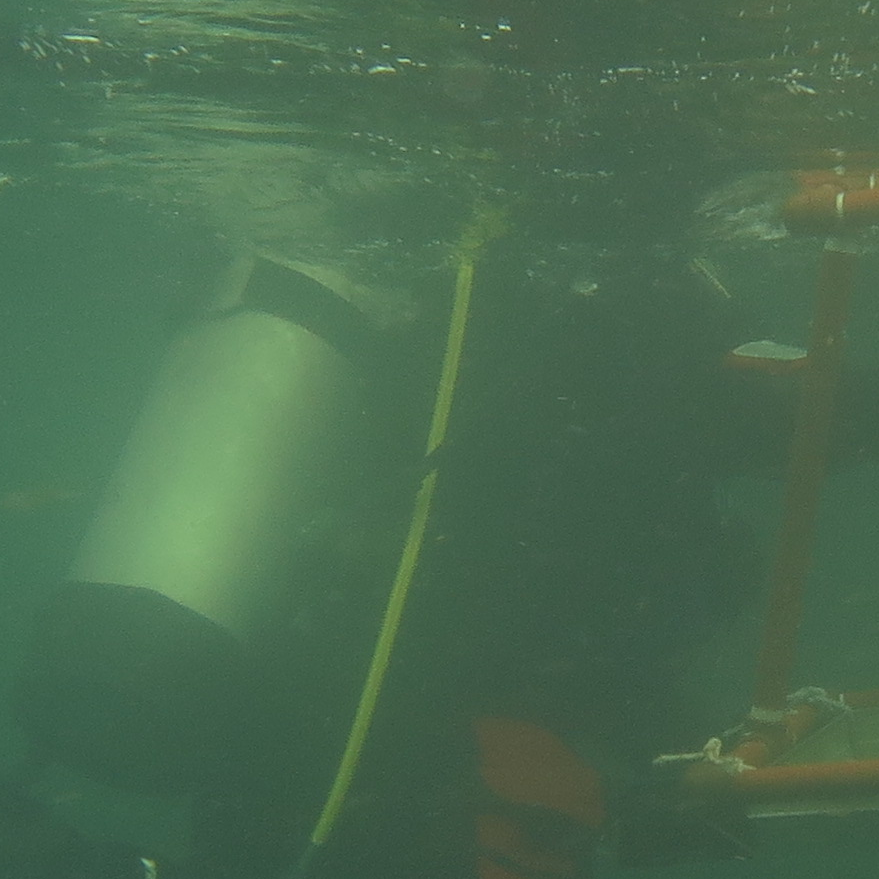
\includegraphics[scale=0.5]{1908xx.png}
    \subcaption{Imagen original}
    \end{subfigure}\hfill
	\begin{subfigure}{0.5\textwidth}
	\centering
        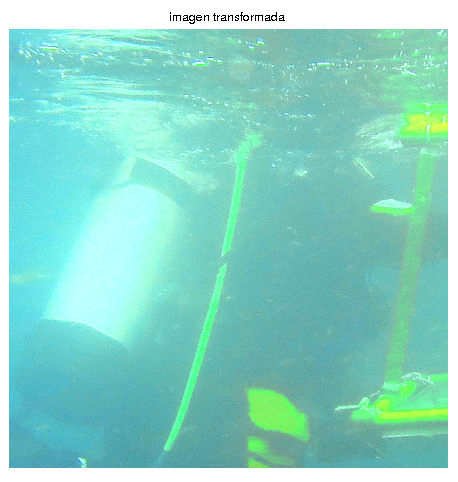
\includegraphics[width=0.9\textwidth]{1923-transformada-40-2x-2x.png}
    \subcaption{Imagen transformada aumentando $40\degree$ H, multiplicado por 2 a S y a I}
    \end{subfigure}\hfill
\end{figure}\hfill

\begin{figure}[H]
	\begin{subfigure}{0.5\textwidth}
	\centering
        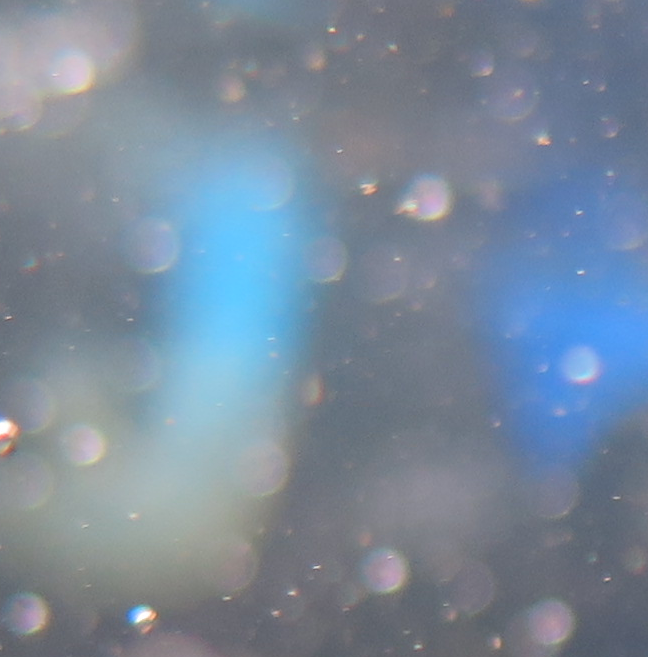
\includegraphics[scale=0.6]{1923xx.png}
    \subcaption{Imagen original}
    \end{subfigure}\hfill
	\begin{subfigure}{0.5\textwidth}
	\centering
        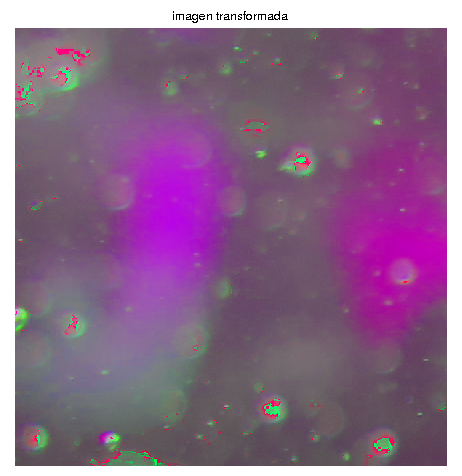
\includegraphics[width=0.9\textwidth]{1923-transformada-90-2x-log.png}
    \subcaption{Imagen transformada aumentando $90\degree$ H, multiplicado por 2 a S y aplicando log(1 + I) a I}
    \end{subfigure}\hfill
\end{figure}\hfill

\section{Realce de saturación}

\subsection{}

El archivo correspondiente a este inciso se llama \textbf{modificarSaturacionDeImagenRGB.m} y toma como parámetro de entrada una imagen en RGB e imprime diversas figuras, cada una mostrando una nueva imagen en RGB cuya saturación fue multiplicada por una constante \textit{c}. Al ejecutar el método, las constantes que se utilizan son las contenidas en el vector $[0.25, 0.5, 0.75, 2, 4, 6]$.

Por ejemplo, al ejecutarlo con la imagen llamada \textit{1908xx.png} y distintos parámetros de \textit{c}, se obtuvieron los siguientes resultados:

\begin{figure}[H]
	\begin{subfigure}{0.5\textwidth}
	\centering
        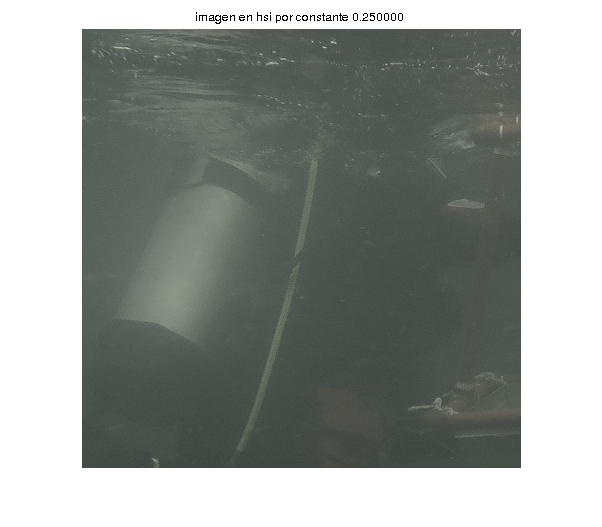
\includegraphics[width=0.9\textwidth]{1908xx-sat-por-025.png}
    \subcaption{$c = 0.25$}
    \end{subfigure}\hfill
	\begin{subfigure}{0.5\textwidth}
	\centering
        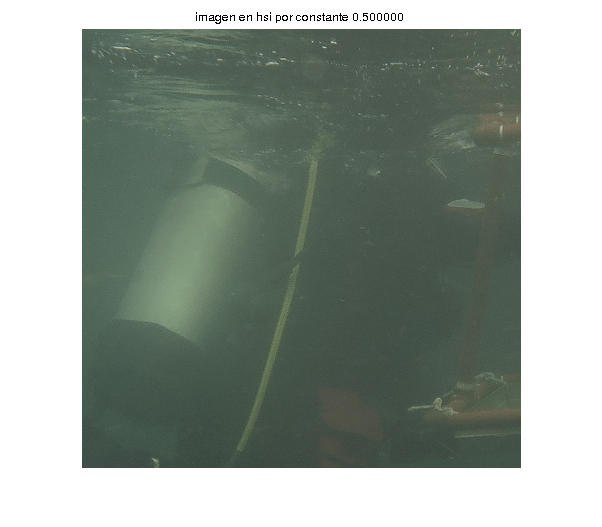
\includegraphics[width=0.9\textwidth]{1908xx-sat-por-050.png}
    \subcaption{$c = 0.50$}
    \end{subfigure}\hfill
	\begin{subfigure}{0.5\textwidth}
	\centering
        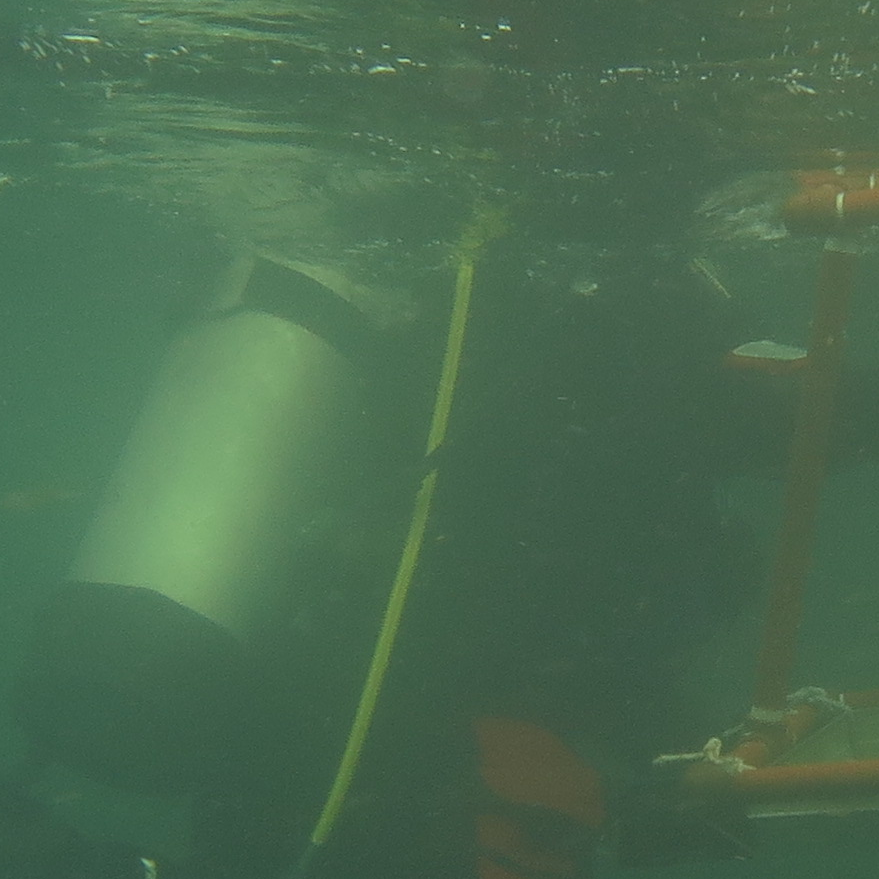
\includegraphics[scale=0.4]{1908xx.png}
    \subcaption{Imagen original}
    \end{subfigure}\hfill
	\begin{subfigure}{0.5\textwidth}
	\centering
        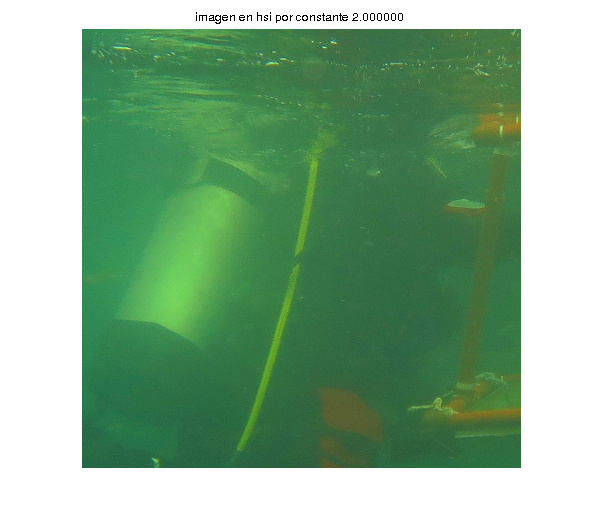
\includegraphics[width=0.9\textwidth]{1908xx-sat-por-2.png}
    \subcaption{$c = 2$}
    \end{subfigure}\hfill
	\begin{subfigure}{0.5\textwidth}
	\centering
        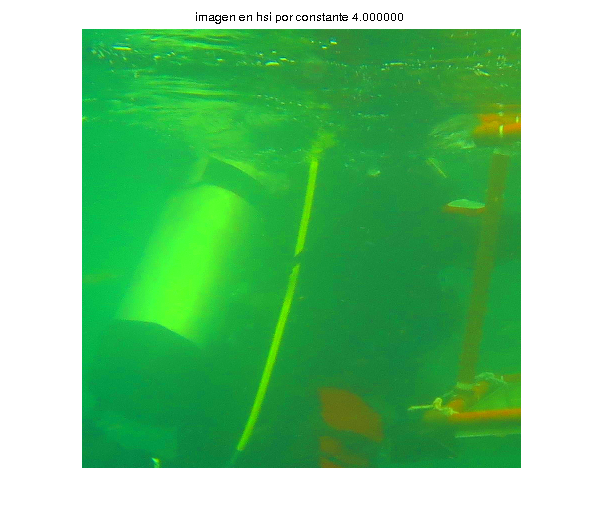
\includegraphics[width=0.9\textwidth]{1908xx-sat-por-4.png}
    \subcaption{$c = 4$}
    \end{subfigure}\hfill
	\begin{subfigure}{0.5\textwidth}
	\centering
        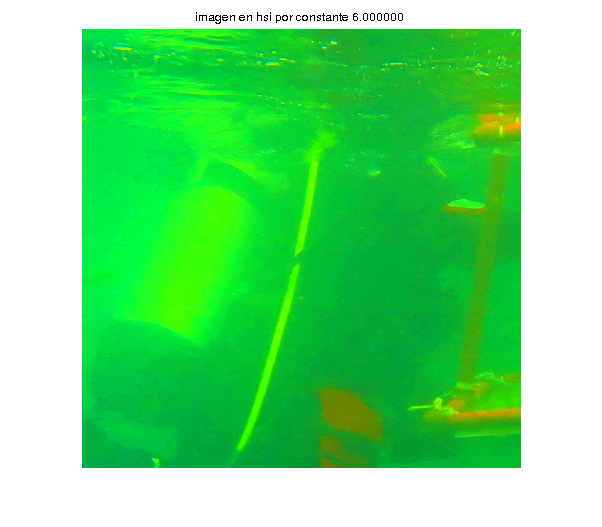
\includegraphics[width=0.9\textwidth]{1908xx-sat-por-6.png}
    \subcaption{$c = 6$}
    \end{subfigure}\hfill
\end{figure}\hfill

\subsection{}

El archivo correspondiente a este inciso se llama \textbf{transformacionesLinealesYNoLinealesAImagenRGB.m} y toma como parámetro de entrada una imagen en RGB y muestra diversas figuras, cada una comparando la imagen original contra una nueva imagen en RGB con una transformación lineal o no lineal sobre el canal de saturación de la imagen en hsi. Realizo cuatro transformaciones distintas:
\begin{itemize}
\item $S = 1 - S$
\item $S = S * S$
\item $S = log(S)$
\item En esta aplico una transformación de forma tal que la saturación vaya aumentando de izquierda a derecha
\item En esta aplico una transformación de forma tal que la saturación vaya aumentando de derecha a izquierda
\end{itemize}

A continuación presento ejemplos de las transformaciones aplicadas a la imagen llamada \textit{1908xxx.png}:

\begin{figure}[H]
	\begin{subfigure}{0.5\textwidth}
	\centering
        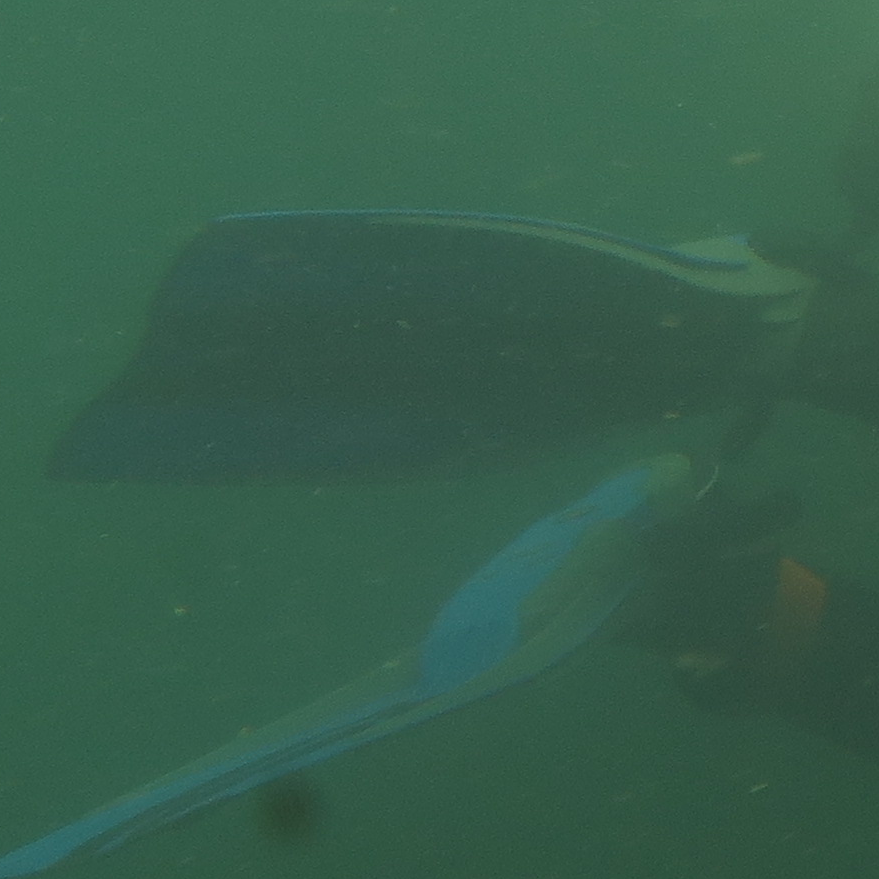
\includegraphics[scale=0.4]{1908xxx.png}
    \subcaption{Imagen original}
    \end{subfigure}\hfill
	\begin{subfigure}{0.5\textwidth}
	\centering
        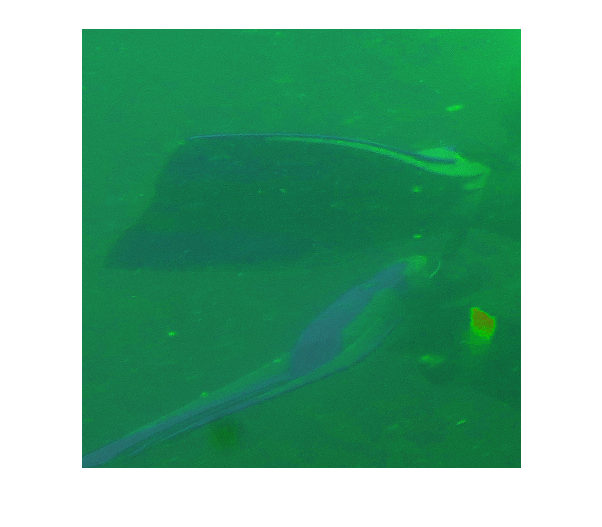
\includegraphics[width=0.9\textwidth]{transf1.png}
    \subcaption{$S = 1 - S$}
    \end{subfigure}\hfill
	\begin{subfigure}{0.5\textwidth}
	\centering
        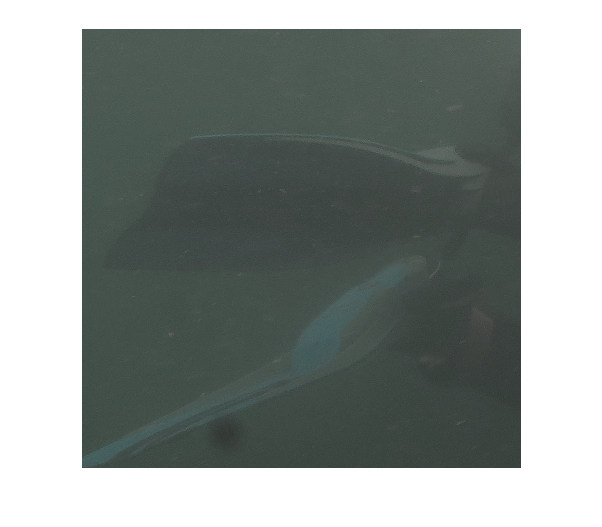
\includegraphics[width=0.9\textwidth]{transf2.png}
    \subcaption{$S = S * S$}
    \end{subfigure}\hfill
	\begin{subfigure}{0.5\textwidth}
	\centering
        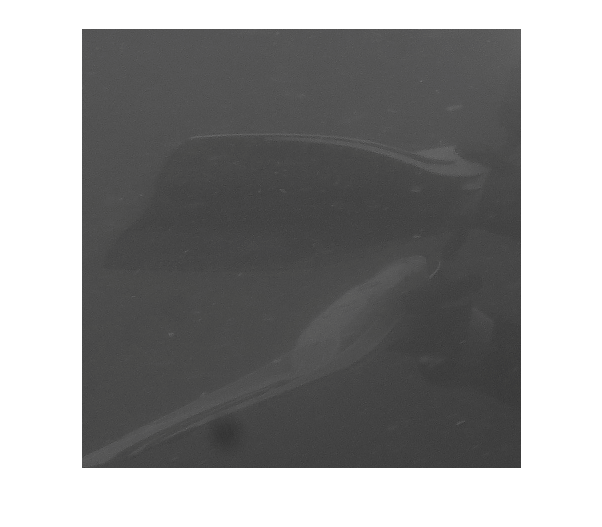
\includegraphics[width=0.9\textwidth]{transf3.png}
    \subcaption{$S = log(S)$}
    \end{subfigure}\hfill
	\begin{subfigure}{0.5\textwidth}
	\centering
        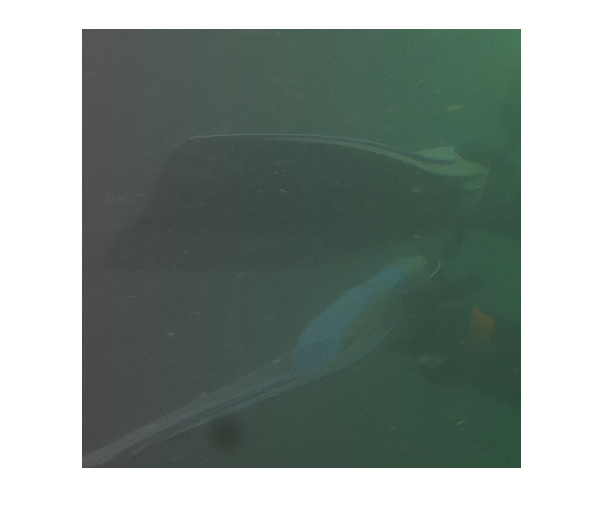
\includegraphics[width=0.9\textwidth]{transf4.png}
    \subcaption{Aumento saturación de izquierda a derecha}
    \end{subfigure}\hfill
	\begin{subfigure}{0.5\textwidth}
	\centering
        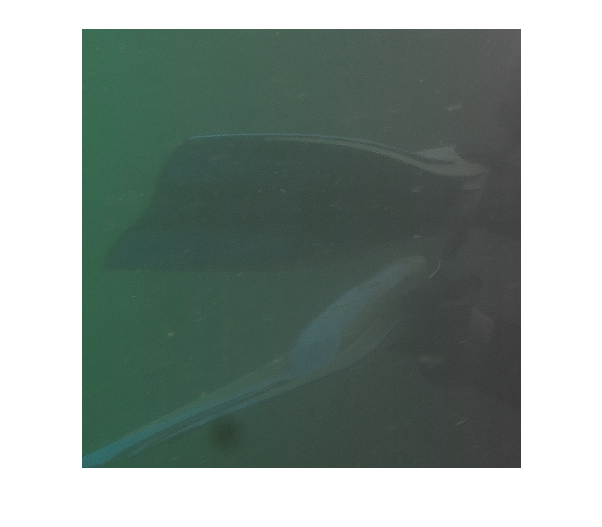
\includegraphics[width=0.9\textwidth]{transf5.png}
    \subcaption{Aumento saturación de derecha a izquierda}
    \end{subfigure}\hfill
\end{figure}\hfill

\section{Alteración de Hue}

El archivo correspondiente a este inciso se llama \textbf{alterarHue.m} y toma como parámetro de entrada una imagen en RGB y muestra diversas figuras, cada una con el valor del canal H aumentado por un valor de $h_{i}$ grados, con $h_{i} \in [20, 45, 60, 90, 140, 180, 240, 300]$.

Por ejemplo, al ejecutarlo con la imagen llamada \textit{1901xx.png} y distintos parámetros de \textit{h}, se obtuvieron los siguientes resultados:

\begin{figure}[H]
	\begin{subfigure}{0.5\textwidth}
	\centering
        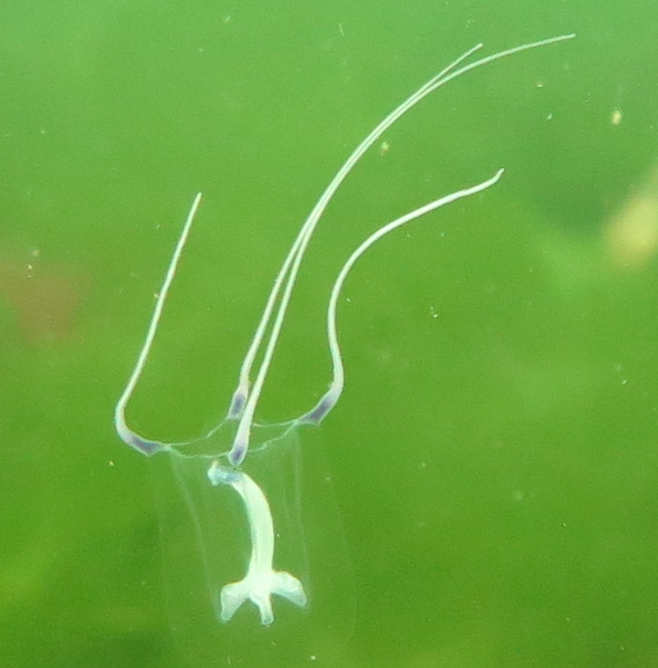
\includegraphics[scale=0.5]{1901xx.png}
    \subcaption{Imagen original}
    \end{subfigure}\hfill
	\begin{subfigure}{0.5\textwidth}
	\centering
        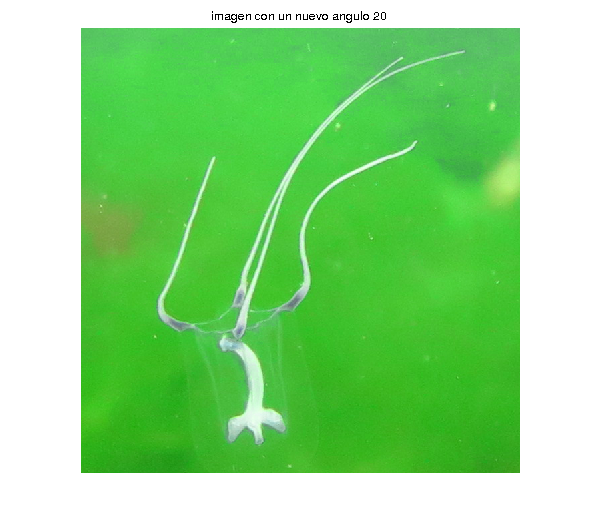
\includegraphics[width=0.9\textwidth]{1901-h-20.png}
    \subcaption{$h_{i} = 20$\degree}
    \end{subfigure}\hfill
	\begin{subfigure}{0.5\textwidth}
	\centering
        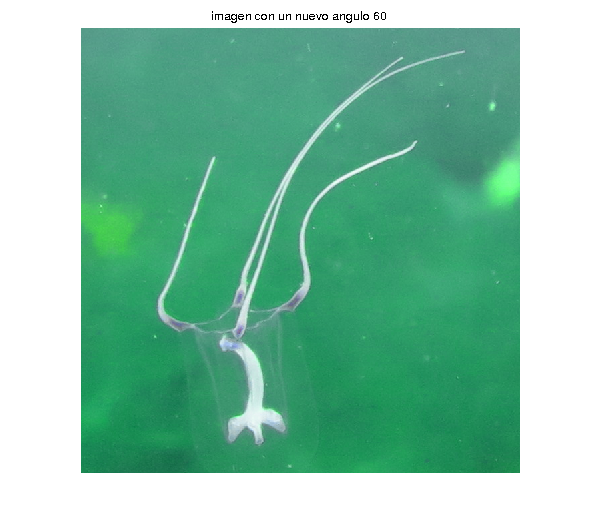
\includegraphics[width=0.9\textwidth]{1901-h-60.png}
    \subcaption{$h_{i} = 60$\degree}
    \end{subfigure}\hfill
	\begin{subfigure}{0.5\textwidth}
	\centering
        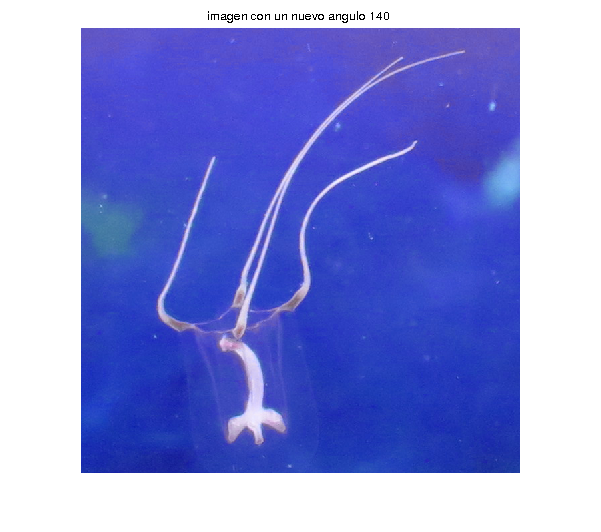
\includegraphics[width=0.9\textwidth]{1901-h-140.png}
    \subcaption{$h_{i} = 140$\degree}
    \end{subfigure}\hfill
	\begin{subfigure}{0.5\textwidth}
	\centering
        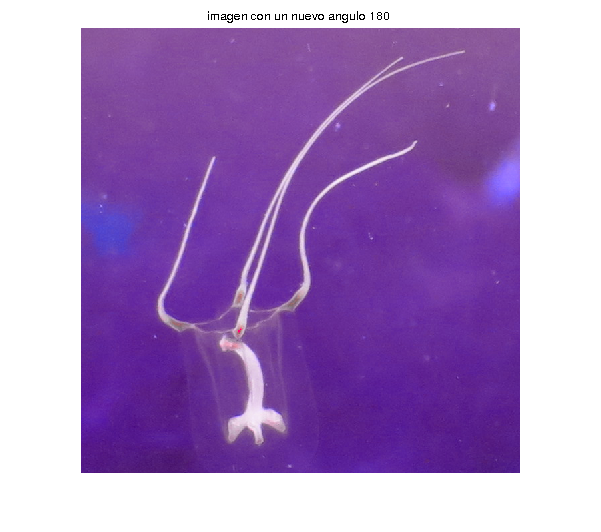
\includegraphics[width=0.9\textwidth]{1901-h-180.png}
    \subcaption{$h_{i} = 180$\degree}
    \end{subfigure}\hfill
	\begin{subfigure}{0.5\textwidth}
	\centering
        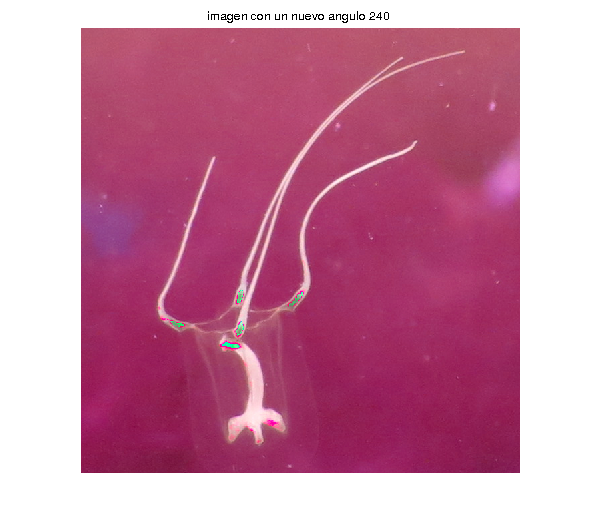
\includegraphics[width=0.9\textwidth]{1901-h-240.png}
    \subcaption{$h_{i} = 240$\degree}
    \end{subfigure}\hfill
\end{figure}\hfill

Se puede observar cómo se va modificando la gama de colores al realizar dicha modificación. La figura del medio de la imagen, al poseer una saturación muy baja, no cambia  mucho su color blanco ya que se puede observar en el modelo, los valores son saturación baja quedan siempre blancos sin importar el valor del Hue. 

\section{HSI}

Luego de analizar varias imágenes proveídas por la cátedra, se puede observar que en el canal I (intensidad) los detalles son más visibles en comparación con el resto. Por ejemplo, a continuación presento una serie de imagénes junto con cada uno de sus canales:

\begin{figure}[H]
	\begin{subfigure}{0.5\textwidth}
	\centering
        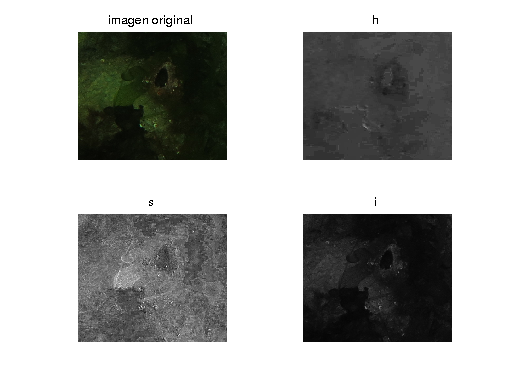
\includegraphics[scale=0.6]{im3.png}
    \subcaption{Imagen 1}
    \end{subfigure}\hfill
	\begin{subfigure}{0.5\textwidth}
	\centering
        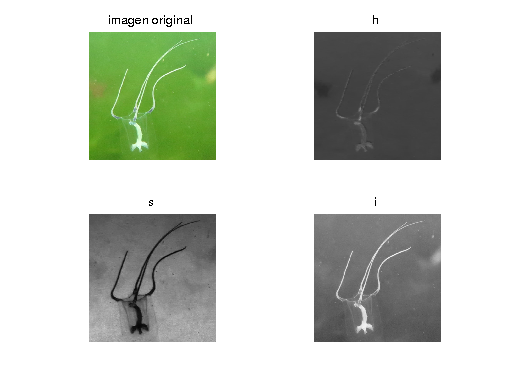
\includegraphics[scale=0.6]{im4.png}
    \subcaption{Imagen 2}
    \end{subfigure}\hfill
	\begin{subfigure}{0.5\textwidth}
	\centering
        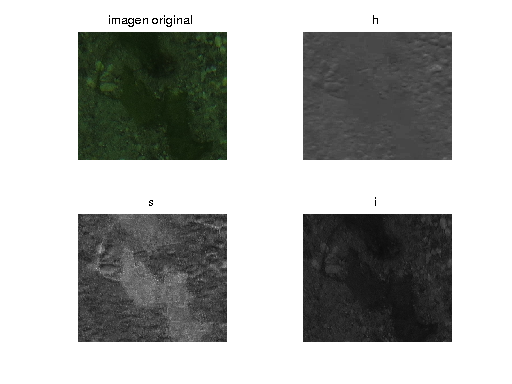
\includegraphics[scale=0.6]{im6.png}
    \subcaption{Imagen 3}
    \end{subfigure}\hfill
	\begin{subfigure}{0.5\textwidth}
	\centering
        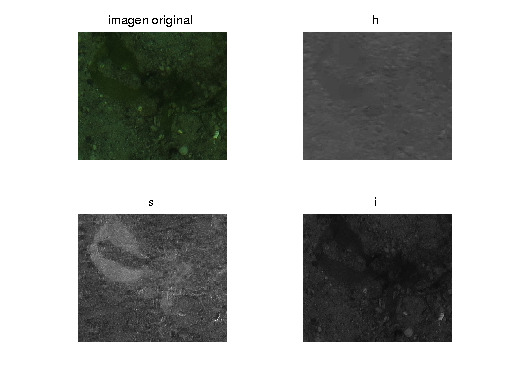
\includegraphics[scale=0.6]{im7.png}
    \subcaption{Imagen 4}
    \end{subfigure}\hfill
	\begin{subfigure}{0.5\textwidth}
	\centering
        \includegraphics[scale=0.6]{im8.png}
    \subcaption{Imagen 5}
    \end{subfigure}\hfill
	\begin{subfigure}{0.5\textwidth}
	\centering
        \includegraphics[scale=0.6]{im9.png}
    \subcaption{Imagen 6}
    \end{subfigure}\hfill
\end{figure}\hfill

Por ejemplo, en la imagen 6, los detalles de líneas blancas en el caño rojo solo se puede distinguir en dicho canal y, en la imagen 1, se pueden distinguir muchos detalles que en los demás canales no se notan. 

En cuanto a la granularidad, ésta se puede distinguir mejor en el canal S (saturación). Además de esto apreciarse en las imágenes anteriores (imagen 1, 3 y 4, por ejemplo), presento otras:

\begin{figure}[H]
	\begin{subfigure}{0.5\textwidth}
	\centering
        \includegraphics[scale=0.6]{im1.png}
    \subcaption{Imagen 7}
    \end{subfigure}\hfill
	\begin{subfigure}{0.5\textwidth}
	\centering
        \includegraphics[scale=0.6]{im2.png}
    \subcaption{Imagen 8}
    \end{subfigure}\hfill
\end{figure}\hfill

Los bordes difuminados afectan notablemente al canal Hue. Aquellos objetos/detalles en las imágenes que poseen bordes difuminados, se puede observar que estos prácticamente no se pueden apreciar en dicho canal. Esto se puede ver en las imágenes anteriores 1 y 7, y sino también se puede observar en la siguiente imagen, en la cual los detalles azules que están difuminados casi desaparecen en este canal: 

\begin{figure}[H]
	\centering
	\begin{subfigure}{0.5\textwidth}
	\centering
        \includegraphics[scale=0.6]{im12.png}
    \subcaption{Imagen 9}
    \end{subfigure}\hfill
\end{figure}\hfill

\end{document}